El objetivo del trabajo será la implementación de un algoritmo de identificación de un sistema fisico determinado. El sistema a identificar puede verse en la figura \ref{fig:auto}, se trata de un sistema de amortiguación de un automovil.

\vspace*{\fill}
\begin{figure}[H]
\centering
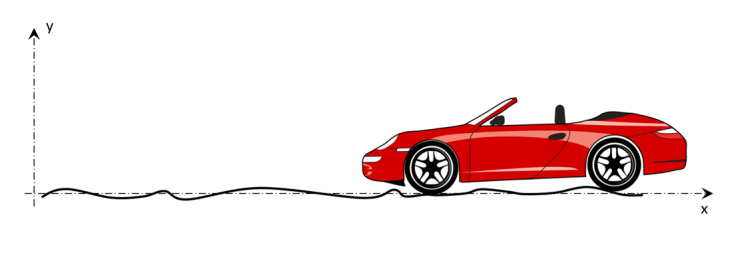
\includegraphics[scale=0.7]{auto.png}
\caption{Sistema Fisico.}
\label{fig:auto} 
\end{figure}
\vspace*{\fill}

El modelo a utilizar para identificar el sistema es el que observamos en la figura \ref{fig:mbk}. Se trata de un sistema de masa, amortiguador y resorte, donde la entrada $x_{1}$ es el nivel del suelo, y la salida $x_{2}$ es la altura en la que se encuentra el chasis del automovil. La idea es, mediante un filtro adaptativo, poder estimar las constantes $m$, $b$ y $k$ del sistema.

\vspace*{\fill}
\begin{figure}[H]
\centering
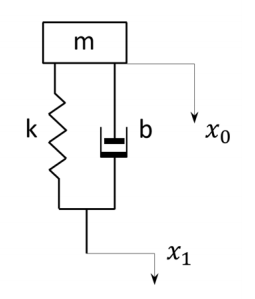
\includegraphics[scale=0.6]{mbk.png}
\caption{Modelo.}
\label{fig:mbk} 
\end{figure}
\vspace*{\fill}
